\hypersetup{pageanchor=false}
\pagestyle{plain}
\renewcommand{\theHsection}{response.\arabic{section}}
\renewcommand{\theHsubsection}{response.\arabic{section}.\arabic{subsection}}
\renewcommand{\theHsubsubsection}{%
  response.\arabic{section}.\arabic{subsection}.\arabic{subsubsection}}
\renewcommand{\theHfigure}{response.\arabic{figure}}
\renewcommand{\theHtable}{response.\arabic{table}}
\renewcommand{\theHequation}{response.\arabic{equation}}

\begin{center}
  {\LARGE\bfseries Response to the Editor and Reviewers\par}
  \vspace{0.6em}
  {\large Manuscript TACO-2026-79:\par}
\end{center}
\vspace{1em}

\noindent Dear Editor-in-Chief, Associate Editor, and Reviewers,

\section{Overall Response}
\label{sec:overall-response}

Thank you for the careful assessment of the manuscript and for the
opportunity to submit a major revision.  The remainder of this response letter
is organized as follows.  Section~2 provides a concise revision map from each
reviewer comment to the corresponding change and location in the revised
manuscript.  Section~3 then responds to each comment in reviewer order.  We
append the marked revised manuscript to this response letter, with links in the
Revision Map and detailed responses pointing directly to the corresponding
manuscript locations.  In the appended manuscript, \DIFdel{xxx} denotes content
from the previous version that has been removed, while \DIFadd{xxx} denotes
content newly added in this revision.

\section{Revision Map}

In the identifiers below, R$x$.$y$ denotes Reviewer $x$'s $y$-th comment; for
example, R2.3 denotes Reviewer~2, Comment~3.

For compact references below, the revised manuscript sections are abbreviated
as follows: \SIntro{} Introduction; \SBG{} Background and Motivation;
\SDesign{} System Design; \SEval{} Evaluation; \SRelated{} Related Work;
\SDiscussion{} Discussion; and \SConclusion{} Conclusion.  The following table
maps every actionable reviewer point to the corresponding revision.

\begingroup
\normalsize
\setlength{\tabcolsep}{1.5pt}
\renewcommand{\arraystretch}{1.18}
\begin{longtable}{@{}>{\raggedright\arraybackslash}p{1.35cm}
                       >{\raggedright\arraybackslash}p{3.75cm}
                       >{\raggedright\arraybackslash}p{7.15cm}
                       >{\raggedright\arraybackslash}p{2.55cm}@{}}
\toprule
\rowcolor{tablehead}
\textbf{ID} & \textbf{Concern} & \textbf{Revision} &
\textbf{Location} \\
\midrule
\endfirsthead
\toprule
\rowcolor{tablehead}
\textbf{ID} & \textbf{Concern} & \textbf{Revision} &
\textbf{Location} \\
\midrule
\endhead
\midrule
\multicolumn{4}{r}{\emph{Continued on the next page}}\\
\endfoot
\bottomrule
\endlastfoot

\responseid{E}{resp:editor} &
Insufficient background, weak evaluation, and unclear novelty relative to
systems such as TileLang. &
Expanded the background and evaluation, including stronger gains in selected
inference scenarios; stated the core challenges and contributions more
precisely. &
\SIntro--\SDiscussion \\
\midrule

\responseid{R1-Q}{resp:r1-q} &
Does ``TilingInfer'' enhance loop tiling? &
Defined TilingInfer as inferring invariant schedule parameters, not searching
for tiling strategies. &
\SIntro \\
\midrule

\responseid{R1.1}{resp:r1-1} &
Add PyTorch, ATen, and Graph IR background. &
Added Graph IR, FX/ATen schemas, and constant-versus-symbolic shape
background. &
\papersec{sec:background:graph-ir} \\
\midrule

\responseid{R1.2}{resp:r1-2} &
Discuss benefits beyond an Ascend NPU with a lean Scalar unit. &
Validated only the footprint effect of pruning a schedule-fixed library on a
non-Ascend platform and bounded the latency claim to Ascend. &
\papersec{sec:eval:tradeoff}; \SDiscussion \\
\midrule

\responseid{R1.3}{resp:r1-3} &
Separate host-control simplification from device-kernel specialization and
show compiler effects beyond loop unrolling. &
Clarified that host code is analyzed, not specialized; attributed gains to
device kernels and documented optimizations beyond loop unrolling. &
\papersec{sec:eval:sensitivity}; \SDiscussion \\
\midrule

\responseid{R1.4}{resp:r1-4} &
Compare a universal static library with per-program pruned libraries. &
Measured a 542\,MB universal archive against 24.3--60.7\,MB per-model
libraries and reported the 8--22-service break-even range. &
\papersec{sec:eval:tradeoff} \\
\midrule

\responseid{R2.1}{resp:r2-1} &
Parameter counts do not show which fields affect performance. &
Added a five-configuration sensitivity study showing that hot-path use sites
matter more than parameter count. &
\papersec{sec:eval:sensitivity} \\
\midrule

\responseid{R2.2}{resp:r2-2} &
Add non-dense-Transformer, model-level evaluation. &
Added six end-to-end scenarios spanning DeepFM, HSTU, Llama 3.2 1B, and
Qwen3.5-0.8B prefill and decode. &
\papersec{sec:eval:setup}; \papersec{sec:eval:result} \\
\midrule

\responseid{R2.3}{resp:r2-3} &
The standard offline-compilation baseline is weak, and the reported
end-to-end gain is too small. &
Enabled NPU Graph Replay, quantified scenario-dependent gains, and added
Optimal as a same-kernel per-shape full-specialization oracle. &
\papersec{sec:eval:setup}; \papersec{sec:eval:result} \\
\midrule

\responseid{R2.4}{resp:r2-4} &
Constant propagation and partial evaluation are established techniques. &
Narrowed the contribution to Graph-IR-to-C++ entry-state construction and
CRVFG early-exit handling, not the compiler passes. &
\SIntro; \papersec{sec:motivation:challenges} \\
\midrule

\responseid{R3.1}{resp:r3-1} &
Clarify the advance over AI compilers such as TileLang and translation tools
such as QiMeng-Xpiler. &
Distinguished in-place specialization and pruning of expert libraries from
generated or translated kernels. &
\SIntro; \SRelated; \SDiscussion \\
\midrule

\responseid{R3.2}{resp:r3-2} &
Add comparisons with AI compilers and libraries such as cuDNN. &
Clarified why no direct comparison is claimed and explained the
cross-implementation and cross-platform confounds. &
\SIntro; \SRelated; \SDiscussion \\
\midrule

\responseid{R3.3}{resp:r3-3} &
Explain accelerator compilation and instruction-translation differences. &
Clarified that TilingInfer does not change GPU/NPU compilation or IR-to-ISA
lowering; no manuscript change was needed. &
No corresponding manuscript location; response only \\
\midrule

\responseid{R3.4}{resp:r3-4} &
The cross-language gap may be only simple parameter passing. &
Defined the type-directed Graph-IR-to-C++ entry mapping; clarified that it is
neither FFI parameter passing nor size-specific optimization. &
\SIntro; \papersec{sec:motivation:challenges} \\
\midrule

\responseid{R3.5}{resp:r3-5} &
What are the rules $\mathcal{R}$ in Fig.~8? &
Defined $\mathcal{R}$ as five type-directed context-update rules, not tiling or
size-selection rules. &
\papersec{sec:design:context_construction},
\paperfig{fig:context_workflow}, and \papertab{tab:semantic-rules} \\
\midrule

\responseid{R3-W}{resp:r3-w} &
The manuscript is difficult to follow and needs clearer English. &
Performed an independent full-paper language check and corrected terminology,
grammar, incomplete phrases, and numerical inconsistencies. &
\SIntro--\SConclusion \\
\end{longtable}
\endgroup

\paragraph{Editorial note.}
To accommodate the added background and experiments within the revision page
limit, we condensed material from the previous manuscript in
\papersec{sec:motivation:auto-spec} and \papersec{sec:eval:analysis}.

\section{Detailed Responses in Reviewer Order}

\reviewcomment{E: Overall assessment}{resp:editor}
{The manuscript needs additional background, a stronger evaluation, and a
clearer account of its core contribution.}

\authorresponse
Thank you for summarizing the main concerns.  We expanded the background on
Graph IR, PyTorch/ATen, and expert-written operator libraries; added
device-level attribution, schedule-parameter sensitivity, six end-to-end
inference scenarios, and a deployment-level binary-size trade-off study; and
reported more pronounced gains in the DeepFM recommendation and LLM-decode
scenarios.  We also revised the statement of the core challenges and
contributions to define their scope and relationship more precisely.  Please
see our responses to
\hyperref[resp:r2-4]{\acmreftext{R2.4 (\S\ref*{resp:r2-4})}} and
\hyperref[resp:r3-4]{\acmreftext{R3.4 (\S\ref*{resp:r3-4})}} for the detailed
contribution boundary.

\loc{\SIntro--\SDiscussion.}

\reviewcomment{R1-Q: Meaning of the name TilingInfer}{resp:r1-q}
{Does TilingInfer aim to enhance loop tiling or related optimizations?}

\authorresponse
``TilingInfer'' refers to using constant propagation on the constant dimensions
and attributes of operator shapes to infer invariant tiling data, i.e.,
schedule parameters, which are then used to specialize or prune kernels.  The
name does not imply that our system searches for or improves loop-tiling
strategies.

To avoid this potential misunderstanding, we added an explanation of the name
to the Introduction.

\loc{\SIntro.}

\reviewcomment{R1.1: PyTorch, ATen, and Graph IR background}{resp:r1-1}
{Please add the background needed to understand calling-context generation.}

\authorresponse
We added a definition of Graph IR and used a PyTorch FX Graph as an example to
explain how Graph IR represents static dimensions and runtime-dynamic
dimensions.  We also explained the parameter mapping between a Graph IR node
and the corresponding operator schema in the underlying operator library,
laying the groundwork for our subsequent design.

\loc{\papersec{sec:background:graph-ir}, ``Graph IR and External Operator
Libraries.''}

\reviewcomment{R1.2: Applicability beyond Ascend}{resp:r1-2}
{Please discuss performance benefits on a wider range of computing systems.}

\authorresponse
On non-Ascend platforms, we validate only the footprint effect of pruning a
schedule-fixed operator library, using FlashInfer on an NVIDIA GPU; we do not
report non-Ascend latency gains.  Performance specialization requires a
schedule-generic expert-written implementation whose schedule parameters remain
runtime variables.  Among the open-source libraries we examined, we did not
find a comparable non-Ascend implementation with the same compilation path for
a controlled latency comparison.  We therefore confine the cross-platform
claim to the library binary-footprint reduction from per-model pruning.

\loc{\papersec{sec:eval:tradeoff}; \SDiscussion, ``Platform applicability.''}

\reviewcomment{R1.3: Host/device breakdown and compiler mechanisms}{resp:r1-3}
{Separate host-side control-flow simplification from device-side
specialization, and examine optimizations beyond loop unrolling.}

\authorresponse
Regarding host/device separation, TilingInfer analyzes host code only to
recover constant schedule parameters and kernel-launch-site reachability; it
neither rewrites nor specializes the host program.  We therefore attribute no
performance gain to host-side control-flow simplification.  We did not design
host specialization because NPU Graph replay suppresses repeated launch
overhead, while identical input shapes across Transformer layers allow
host-computed schedule parameters to be reused.  Host schedule computation is
therefore not a bottleneck in our evaluated setting.  Moreover,
operator-library code bloat arises mainly from enumerated device-kernel
template instances.

The device kernel's lower-level compiler on Ascend is closed source, and we currently
have neither source access nor permission to modify it.  We therefore cannot
disable loop unrolling alone and must use the default optimization-pass
pipeline for all compared variants.

To examine benefits beyond loop unrolling under this constraint, we conduct a controlled sensitivity 
analysis in \papersec{sec:eval:sensitivity} and \paperfig{fig:eval:constant-sensitivity} by specializing different groups of schedule parameters. 
The results show benefits from simplifying control flow, address calculations, task assignment, and buffer management, not only from loop unrolling. 


\loc{\papersec{sec:eval:sensitivity};
\paperfig{fig:eval:constant-sensitivity}; \SDiscussion.}

\reviewcomment{R1.4: Universal archive versus per-model binaries}{resp:r1-4}
{A separate custom library for every program may consume more total storage
than one universal static library.}

\authorresponse
We added a deployment-level FlashInfer study.  The universal AOT-compiled
library occupies 542\,MB.  Across 17 model variants, the corresponding
per-model pruned libraries occupy 24.3--60.7\,MB, an 88.8--95.5\%
reduction.  Without cross-service deduplication, per-model pruning
remains beneficial for up to eight model services in the worst case and up to
22 in the best case.  Shared container layers, deduplication, and model mix can
shift this break-even point.  We therefore conclude that universal operator
libraries remain attractive for highly diverse shared deployments, whereas
per-model pruning is useful for isolated containers and modest model sets.

\loc{\papersec{sec:eval:tradeoff}, ``Binary-Size Trade-off.''}

\reviewcomment{R2.1: Sensitivity to individual parameters}{resp:r2-1}
{Counting resolved fields does not show which fields actually influence
hardware stalls or performance.}

\authorresponse
We agree and added a sensitivity study of the benefits of specializing
scheduling parameters for the Flash Attention operator.  The results are:

\begin{itemize}[leftmargin=*,nosep]
  \item Control logic, 6 scheduling parameters: 1.02$\times$.
  \item Per-core tile dimensions and addressing, 14 scheduling parameters:
  1.04$\times$.
  \item Core-loop scheduling and memory resources, 14 scheduling parameters:
  1.07$\times$.
  \item The three groups jointly, 34 scheduling parameters: 1.10$\times$.
  \item All constant schedule parameters specialized by TilingInfer, 352
  parameters: 1.14$\times$.
\end{itemize}

For the evaluated D-Attn implementation and shapes, specializing the 34
hot-path parameters above achieves 75.0\% of TilingInfer's full gain, while the
remaining 318 parameters contribute only an additional 3.4 percentage points.
Within this scope, the types and use sites of the specialized schedule
parameters matter more than their number.

\loc{\papersec{sec:eval:sensitivity}, ``Sensitivity to Resolved Schedule
Parameters.''}

\reviewcomment{R2.2: Non-dense-Transformer evaluation}{resp:r2-2}
{Please add model-level evidence from CV or recommendation architectures.}

\authorresponse
We expanded the evaluation to six representative end-to-end inference
scenarios: DeepFM recommendation, HSTU generative recommendation, Llama 3.2 1B
prefill and decode, and Qwen3.5-0.8B prefill and decode.  For all six scenarios,
we report end-to-end speedup, device-kernel category composition, and
category-level specialization speedup.

\loc{\papersec{sec:eval:setup} and \papersec{sec:eval:result}.}

\reviewcomment{R2.3: Magnitude and baselines}{resp:r2-3}
{The reported end-to-end improvement is too small, and standard offline
compilation is a weak baseline.}

\authorresponse
Across six representative inference scenarios, TilingInfer achieves a
1.05$\times$ geometric-mean end-to-end speedup. Gains are lower for the
compute-intensive HSTU and LLM prefill scenarios, where tensor computation
dominates. In contrast, DeepFM and the two LLM decode scenarios average
1.10$\times$ because their shorter, relatively memory-intensive kernels expose
a larger fraction of removable scalar and scheduling overhead.

The average gain of the two decode scenarios increased from approximately 3\%
in the previous manuscript to 10\% after we enabled NPU Graph replay for all
compared methods. This suppresses repeated CPU launch overhead that previously
masked the contribution of device-kernel specialization.

To address the baseline concern, we compare TilingInfer with Optimal, a
per-shape full-specialization oracle that specializes all schedule parameters
produced by host scheduling. Although impractical for production because it
recompiles every shape, Optimal provides a same-kernel reference. TilingInfer
and Optimal average 1.05$\times$ and 1.08$\times$ across all six scenarios,
and 1.10$\times$ and 1.14$\times$ across the two decode scenarios,
respectively. Each data point averages 90 measured runs after 10 warm-up runs
to reduce measurement noise.

\loc{\papersec{sec:eval:setup} and \papersec{sec:eval:result}.}

\reviewcomment{R2.4: Classical partial evaluation and constant
propagation}{resp:r2-4}
{The work appears to integrate established compiler techniques rather than
introduce a new concept.}

\authorresponse
We agree that constant propagation, partial evaluation, and template
instantiation are mature techniques, and we do not claim these compiler passes
themselves as novel.  TilingInfer's contribution is to establish two
prerequisites missing when applying these techniques to expert-written
operator libraries.

First, although runtime FFI can pass concrete tensor and attribute values, it
does not expose the distinction between model constants and symbolic dimensions
in Graph IR as compile-time facts usable by a separately compiled C++/LLVM
operator library.  For example, both dimensions of the Graph IR shape
\texttt{[s\_B, 40]} appear as integer loads through
\texttt{Tensor::size(i)} after entering C++.  TilingInfer uses type-directed
context-update rules to materialize 40 as a constant and preserve
\texttt{s\_B} as unknown in the C++ entry state, without analyzing Python/C++
FFI glue code.  These rules cover five core parameter types and their standard
nested compositions and are not written for specific sizes.

Second, TilingInfer uses CRVFG to identify early-exit edges in shape checkers
before constant propagation, preventing error paths from polluting the analysis
state of normal paths while avoiding full path-sensitive analysis.  Thus, the
contribution is not a new partial-evaluation theory, but cross-layer entry-state
construction and early-exit identification mechanisms that enable existing
compiler optimizations to be applied to expert-written operator libraries.  We
have clarified this contribution boundary in the revised manuscript.

\loc{\SIntro{} contribution statement;
\papersec{sec:motivation:challenges}, ``Challenges and Design Insights.''}

\reviewcomment{R3-W: Clarity and English expression}{resp:r3-w}
{The manuscript is difficult to follow, and the English should be refined.}

\authorresponse
Thank you for this comment on the presentation.  We performed an independent
full-paper language check in addition to reorganizing the manuscript.  The
revision standardizes terminology and examples and corrects subject--verb
agreement, incomplete phrases, awkward constructions, and numerical
inconsistencies throughout.

\loc{Substantial revisions throughout \SIntro--\SConclusion.}

\reviewcomment{R3.1: AI compilers, TileLang, and QiMeng-Xpiler}{resp:r3-1}
{The manuscript should explain what remains distinctive relative to AI
compilers and code-translation tools.}

\authorresponse
These approaches share the ultimate goal of improving operator performance, but
differ in their optimization targets and compilation paths.  AI compilers such
as TileLang start from high-level operator descriptions and generate new
specialized kernels through multi-level IRs, schedule search, or autotuning.
Code-translation tools such as QiMeng-Xpiler use LLM-based transformations,
symbolic repair, and tuning to generate or port target implementations.

TilingInfer neither regenerates operator implementations nor searches for new
scheduling strategies.  Instead, it targets existing expert-written operator
libraries and introduces constants from Graph IR into their C++/LLVM
compilation flows to perform partial evaluation on kernels and prune unreachable
precompiled instances.

Thus, TilingInfer's advance lies in providing existing expert-written operator
libraries with automatic specialization and pruning capabilities across Graph
IR and C++/LLVM.  It takes a different but complementary technical path from
the generative approaches above.

We added an explanation of these distinctions to the Introduction and Related
Work.

\loc{\SIntro; \SRelated, ``AI Compilers and Kernel Generation'';
\SDiscussion.}

\reviewcomment{R3.2: Comparisons with AI compilers and cuDNN}{resp:r3-2}
{The evaluation should compare against existing AI compilers and specialized
libraries such as cuDNN.}

\authorresponse
We carefully considered this comment but concluded that TilingInfer should not
be compared directly with AI compilers or specialized libraries such as cuDNN.

For AI compilers, as discussed in our response to R3.1, the scheduling
implementations of AI-compiler-generated kernels differ from those in the
expert-written operator libraries optimized by TilingInfer.  A direct
comparison would therefore conflate the benefits of specialization with
performance differences in the kernels' own scheduling implementations.  To
illustrate this gap, we additionally measured TileLang-Ascend and the CANN
expert-written operator library on Ascend, as shown in
\hyperref[fig:tilelang-cann-roofline]{%
  \acmreftext{Fig.~\ref*{fig:tilelang-cann-roofline}}}:

\begin{itemize}[leftmargin=*,nosep]
  \item Grouped Matmul: CANN averages 100.2\,TFLOPS, while TileLang-Ascend
  averages 28.2\,TFLOPS.
  \item Matmul: CANN averages 173.6\,TFLOPS, while TileLang-Ascend averages
  97.0\,TFLOPS.
\end{itemize}

We did not compare against well-known specialized libraries such as cuDNN for
two reasons:

\begin{enumerate}[label=(\arabic*),leftmargin=*,nosep]
  \item Our operator partial-evaluation experiments are conducted on Ascend,
  whereas cuDNN targets NVIDIA GPUs, making a direct cross-platform comparison
  difficult.  Our response to R1.2 discusses in detail why the operator
  partial-evaluation experiments are based on Ascend.

  \item For pruning precompiled operator instances, cuDNN's core library is
  closed source.  TilingInfer cannot obtain its LLVM IR and therefore cannot
  optimize cuDNN itself.  A direct library-size comparison between FlashInfer
  and specialized libraries such as cuDNN would likewise be difficult to
  interpret.
\end{enumerate}

Moreover, CANN and FlashInfer, the two operator libraries optimized in this
work, are both expert-written libraries widely used in production.
State-of-the-art inference engines provided by open-source communities or
hardware vendors, including vLLM/vLLM-Ascend, SGLang/SGLang-Ascend, and MindIE,
use these libraries by default.

\begin{figure}[H]
  \centering
  \begin{minipage}[t]{0.49\linewidth}
    \centering
    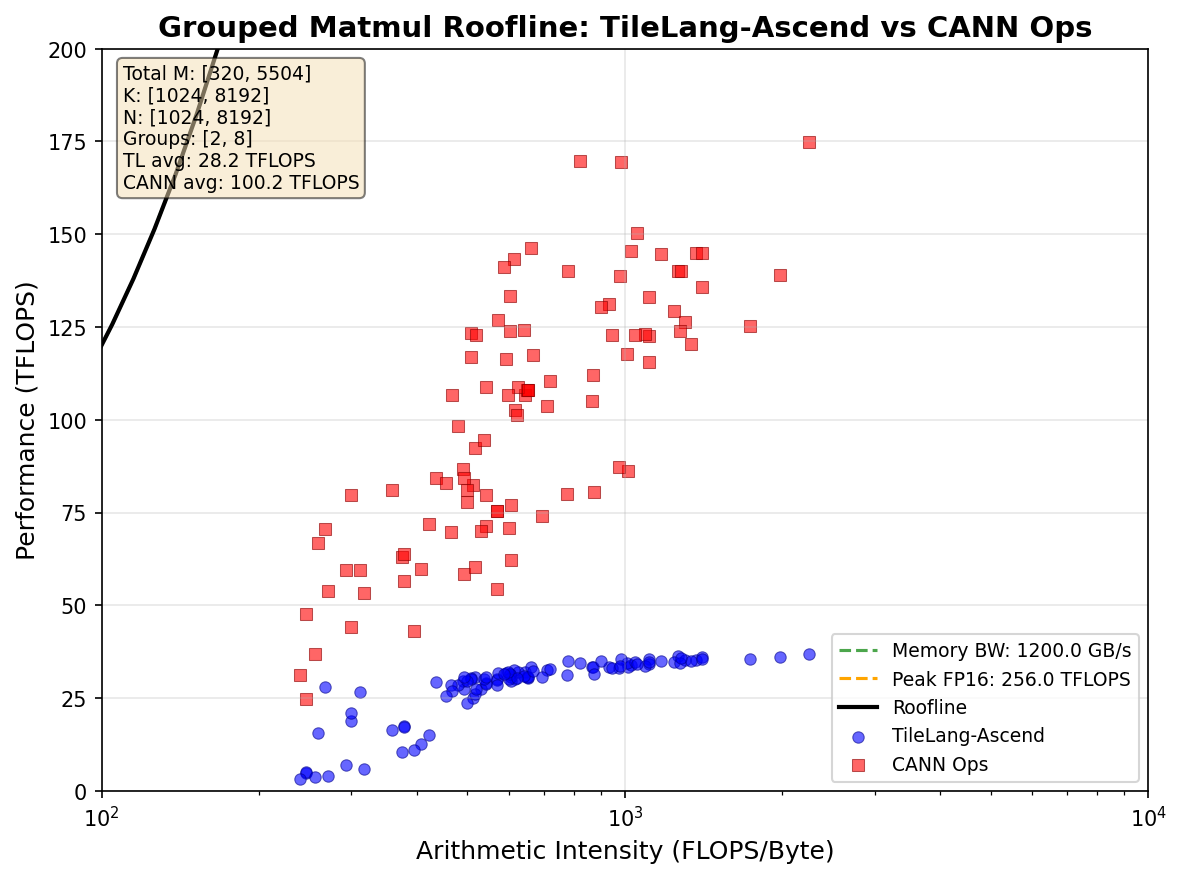
\includegraphics[width=\linewidth]{response_letter/figures/tilelang-vs-cann-gmm.png}
  \end{minipage}\hfill
  \begin{minipage}[t]{0.49\linewidth}
    \centering
    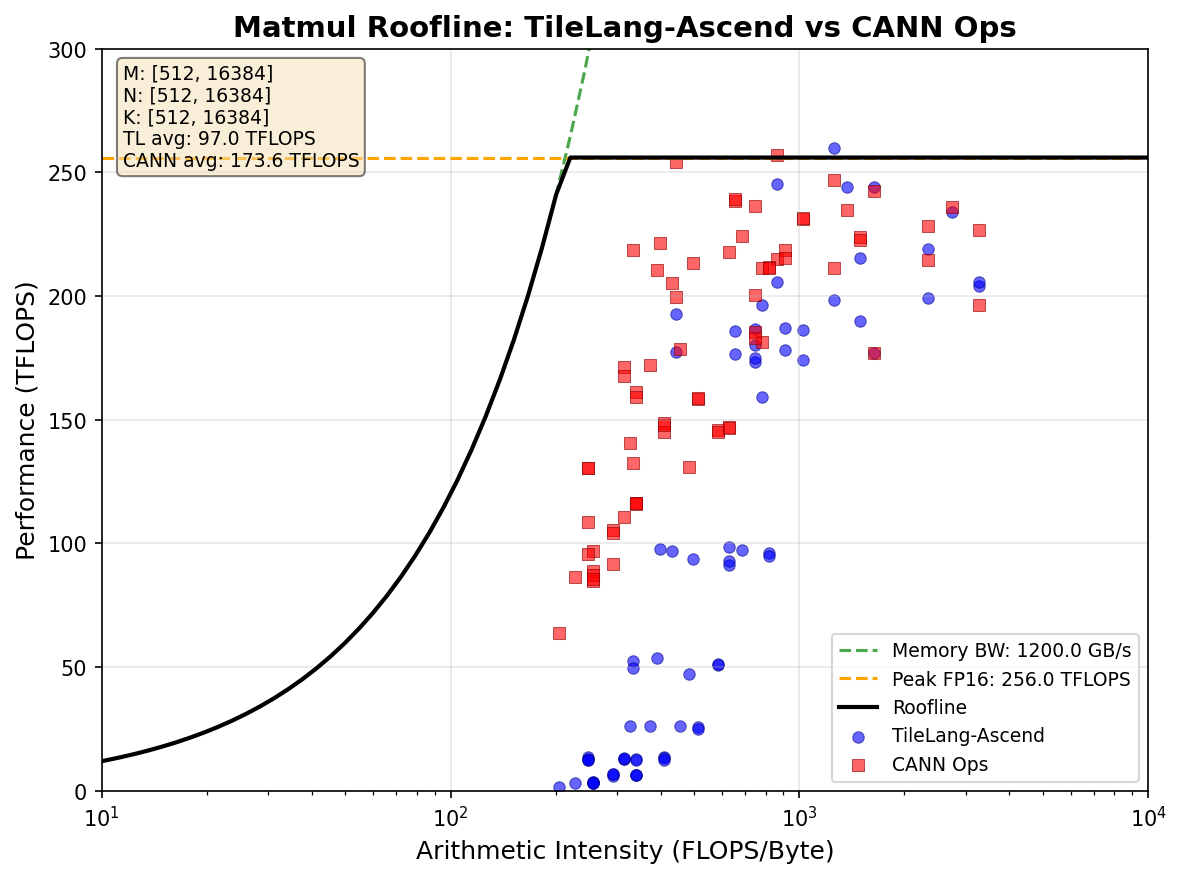
\includegraphics[width=\linewidth]{response_letter/figures/tilelang-vs-cann-mm.png}
  \end{minipage}
  \caption{Ascend roofline characterization of CANN and TileLang-Ascend for
  Grouped Matmul (left) and Matmul (right).}
  \Description{Two Ascend roofline scatter plots comparing TileLang-Ascend and
  CANN for Grouped Matmul and Matmul across sampled arithmetic intensities.}
  \label{fig:tilelang-cann-roofline}
  \vspace{-4pt}
\end{figure}

\loc{\SIntro; \SRelated; \SDiscussion.  The roofline plots above are included only in this
response and were not added to the manuscript.}

\reviewcomment{R3.3: NPU and GPU compilation paths}{resp:r3-3}
{The design should explain compilation and instruction translation for the
two accelerators.}

\authorresponse
TilingInfer operates within the compilation flow of existing expert-written
libraries.  It analyzes and transforms LLVM IR emitted from their C++ host and
device implementations, but it does not modify the subsequent
backend-specific lowering from compiler IR to GPU or NPU machine instructions.
The existing accelerator backend and instruction-selection pipelines remain
unchanged.

Because backend instruction lowering is outside TilingInfer's optimization
scope and is not required to explain its cross-layer constant propagation, we
did not add backend-lowering details to the manuscript.

\loc{No corresponding manuscript location; response clarification only.}

\reviewcomment{R3.4: Is the cross-language gap a real challenge?}{resp:r3-4}
{Determining tensor shapes and attributes may appear to be a collection of
independent size-specific optimizations followed by simple integration.}

\authorresponse
Thank you for identifying the ambiguity.  Inferring tensor shapes and operator
attributes is not itself a contribution of this work; systems such as Dynamo
and TVM Relax already provide symbolic shape inference.  The challenge is to
materialize the constants and symbolic information available in Graph IR into
an entry state that C++/LLVM analysis can use.

Runtime FFI can pass concrete tensor-shape and operator-attribute values, but it
does not preserve the distinction between constant and symbolic dimensions in
Graph IR as compile-time information usable by a separately compiled operator
library.  After entering C++, parameters such as Tensor, List, and Optional are
represented as composite objects with nested memory layouts, and their accesses
are lowered to pointer arithmetic and field loads.  End-to-end cross-language
static analysis would also need to process framework dispatch, type conversion,
object construction, value copying, reference counting, and other FFI code
unrelated to the target mapping, making the analysis expensive and
framework-specific.

TilingInfer defines type-directed context-update rules for the five core
parameter types Scalar, String, Tensor, List, and Optional.  These rules
directly materialize Graph IR metadata as abstract states at the corresponding
C++ object fields and memory locations, while recursive rules support standard
nested compositions.  The rules are selected by parameter type rather than
concrete size: TilingInfer neither enumerates shapes nor implements separate
optimizations for different sizes, but instead propagates the recovered
constants through the same C++/LLVM implementation to kernel launch sites.

Therefore, this process is neither simple parameter passing nor a collection
of independent size-specific optimizations.

\loc{\SIntro; \papersec{sec:motivation:challenges},
``Challenges and Design Insights.''}

\reviewcomment{R3.5: Meaning of the rules
\texorpdfstring{$\mathcal{R}$}{R}}{resp:r3-5}
{What do the rules in Fig.~8 represent, and are they optimizations for
different operator sizes?}

\authorresponse
These rules are neither tiling rules nor size-selection rules.  They are
mappings from Graph IR to C++ memory objects for five basic operator parameter
types: Scalar, String, Tensor, List, and Optional.  For the metadata of a given
Graph IR node, the rules define how to construct the C++ entry state.

To avoid reader confusion, we revised the workflow text and title in Fig.~8,
introduced the meaning of the rule family $\mathcal{R}$ at the beginning of
Section~3.2, and listed the symbol for each rule in Table~2 so that the role of
$\mathcal{R}$ is explicit.

\loc{\papersec{sec:design:context_construction}, especially
\paperfig{fig:context_workflow} and \papertab{tab:semantic-rules}.}

\enlargethispage{3\baselineskip}
\noindent Sincerely,\\
on behalf of all authors
